\documentclass[a4paper, 11pt]{article}
\usepackage[top=3cm, bottom=3cm, left = 2cm, right = 2cm]{geometry} 
\geometry{a4paper} 
\usepackage[utf8]{inputenc}
\usepackage{textcomp}
\usepackage{graphicx} 
\usepackage{amsmath,amssymb}  
\usepackage{bm}  
\usepackage[pdftex,bookmarks,colorlinks,breaklinks]{hyperref}  
\hypersetup{linkcolor=black,citecolor=black,filecolor=black,urlcolor=black} % black links, for printed output
\usepackage{memhfixc} 
\usepackage{pdfsync}  
\usepackage{fancyhdr}
\usepackage{listings}
\usepackage{xcolor}
\usepackage{float}

\definecolor{codegray}{rgb}{0.5,0.5,0.5}
\definecolor{codegreen}{rgb}{0,0.6,0}
\definecolor{codeblue}{rgb}{0.26,0.53,0.96}

\lstset{ 
  backgroundcolor=\color{white},   
  basicstyle=\ttfamily\footnotesize,
  breakatwhitespace=false,         
  breaklines=true,                 
  captionpos=b,                    
  commentstyle=\color{codegreen},
  escapeinside={\%*}{*)},          
  keywordstyle=\color{codeblue},
  stringstyle=\color{codegray},
  showspaces=false,
}
\pagestyle{fancy}
\setlength{\headheight}{13.6pt}

\title{Movers \\[1ex] \large Theory of Computation, Spring 2024}
\author{Luca Di Bello, Agnese Zamboni, Dimitrios Pagonis, Georgy Batyrev} 
\date{\today}

\begin{document}
\maketitle
\tableofcontents

\pagebreak

\section{Problem Description}

In the \textit{movers satisfiability problem}, a moving company is tasked with relocating all furniture from a building with multiple floors. The objective is to move all furniture to the ground floor within a given time frame (maximum number of time steps). For this task, the company has a team of movers of size $m$, and each mover is identified with a unique name, and can move up or down one floor at a time.

The building has $n$ floors, each identified by a unique integer number. The building contains a set of furniture $F = {f1,f2,...,fn}$ to be moved. Each piece of furniture is located within the floors of the building, and there could be more than one piece of furniture on the same floor. The movers are initially located on the ground floor of the building, and they must move all furniture to the ground floor within a given time frame. By the end of the time frame, all movers and all furniture must be located on the ground floor in order to solve the problem.

When a mover is on the same floor as a piece of furniture, and decides to carry it, the mover and the furniture in question are moved together to the floor below.

\pagebreak

\section{Mathematical representation}

\subsection{Input Parameters}

\begin{enumerate}
	\item $m \in \mathbb{N}^+$: number of movers
	\item $n \in \mathbb{N}^+$: number of floors
	\item $t_{max} \in \mathbb{N}^+$: maximum number of steps to solve the problem
\end{enumerate}

\subsection{Sets / Domains}

\begin{itemize}
	\item $M = \{m_1, m_2, ..., m_m\}$: set of movers
	\item $L = \{l_1, l_2, ..., l_n\}$: set of floors ("levels") in the building
	\item $F = \{f_1, f_2, ..., f_k\}$: set of forniture items
	\item $T = \{t_1, t_2, ..., t_{max}\}$: set of timestamps from 1 to $t_{max}$
\end{itemize}


\subsection{Variables}

\subsubsection{Variables describing the state of the system}

\begin{itemize}
	\item $atFloor(m, l, t) \in \{0, 1\}$, \textit{True} if mover $m$ is at floor $l$ at time $t$
	\item $atFloorForniture(f, l, t) \in \{0, 1\}$, \textit{True} if forniture $f$ is at floor $l$ at time $t$
\end{itemize}

\subsubsection{Variables describing the actions of the movers}

\begin{itemize}
	\item $ascend(m, t) \in \{0, 1\}$, \textit{True} if mover $m$ is ascending at time $t$
	\item $descend(m, t) \in \{0, 1\}$, \textit{True} if mover $m$ is descending at time $t$
	\item $carry(m, f,  t) \in \{0, 1\}$, \textit{True} if mover $m$ is carrying forniture $f$ at time $t$
\end{itemize}

\subsection{Constraints}

\subsubsection{Action Definition}

This section describes how the actions of the movers alter the state of the system.

\begin{enumerate}
	\item $ascend(m, t)$: a mover can move up one floor at a time (except when at the last floor)
	      $$
		      l < n -1 \land atFloor(m, l, t) \land ascend(m, t) \implies atFloor(m, l+1, t+1)
	      $$
	      $\forall$ mover $m \in M$, floor $l \in L$, time $t \in T$

	\item $descend(m, t)$: a mover can move down one floor at a time (except when at the ground floor)
	      $$
		      l > 0 \land atFloor(m, l, t) \land descend(m, t) \implies atFloor(m, l-1, t+1)
	      $$
	      $\forall$ mover $m \in M$, floor $l \in L$, time $t \in T$

	\item $carry(m, f, t)$: a mover can carry a piece of forniture if it is at the same floor as the mover. At the next time step, the mover and the forniture will be at the floor below (except when at the ground floor):
	      \begin{align*}
		      l > 0 \land atFloor(m, l, t) \land atFloorForniture(f, l, t) \land carry(m, f , t) & \implies \\
		      atFloor(m, l-1, t+1) \land atFloorForniture(f, l-1, t+1)
	      \end{align*}
	      $\forall$ mover $m \in M$, forniture $f \in F$, floor $l \in L$, time $t \in T$

\end{enumerate}


\subsubsection{Initial and Final Constraints}

\begin{enumerate}
	\item Initial constraint: movers start at the ground floor

	      $$atFloor(m_i, 0, 0)$$

	      $\forall$ mover $m \in M$

	\item Final constraint: movers end at the ground floor

	      $$atFloor(m, 0, t_{max}) \land atFloorForniture(f, 0, t_{max})$$

	      $\forall$ mover $m \in M$, forniture $f \in F$



\end{enumerate}

\subsubsection{Other Constraints}

\begin{enumerate}
	\item Each mover is exactly at one floor at a time

	      \begin{itemize}
		      \item Each mover is at least at one floor
		            $$ \bigvee_{m \in M, l \in L, t\in T} atFloor(m, l, t) $$

		      \item A mover cannot be at more than one floor
		            $$ atFloor(m, l_1, t) \implies \lnot atFloor(m, l_2, t) $$

		            $\forall$ mover $m \in M$, floors $l_1 \neq l_2 \in L$, time $t \in T$
	      \end{itemize}

	\item Each forniture is exactly at one floor at a time

	      \begin{itemize}
		      \item Each forniture is at least at one floor
		            $$ \bigvee_{f \in F, l \in L, t\in T} atFloorForniture(f, l, t) $$

		      \item A forniture cannot be at more than one floor
		            $$ atFloorForniture(f, l_1, t) \implies \lnot atFloorForniture(f, l_2, t) $$

		            $\forall$ forniture $f \in F$, floors $l_1 \neq l_2 \in L$, time $t \in T$
	      \end{itemize}

	\item If a mover is not ascending, descending, or carrying it stays at the same floor

	      $$atFloor(m,l,t) \land \lnot ascend(m, t) \land \lnot descend(m, t) \land \bigwedge_{f \in F} \lnot carry(m, f, t) \implies atFloor(m,l, t+1) $$

	      $\forall$ mover $m \in M$, floor $l \in L$, time $t \in T$

	\item If a forniture is not being carried, it stays at the same floor

	      $$atFloorForniture(f, l, t) \land \bigwedge_{m \in M} \lnot carry(m, f, t) \implies atFloorForniture(f, l, t + 1)$$

	      $\forall$ forniture $f \in F$, floor $l \in L$, time $t \in T$

	\item Each mover can do only one action at a time

	      \begin{itemize}
		      \item $ascend(m, t) \implies \lnot descend(m, t)$
		      \item $ascend(m, t) \implies \lnot carry(m, f, t)$
		      \item $descend(m, t) \implies \lnot ascend(m, t)$
		      \item $descend(m, t) \implies \lnot carry(m, f, t)$
		      \item $carry(m, f, t) \implies \lnot ascend(m, t)$
		      \item $carry(m, f, t) \implies \lnot descend(m, t)$
	      \end{itemize}

	      $\forall$ mover $m \in M$, floor $l \in L$, forniture $f \in F$, time $t \in T$

	\item Each mover can carry at most one piece of forniture

	      $$ carry(m, f_1, t) \implies \lnot carry(m, f_2, t)$$

	      $\forall$ mover $m\in M$, forniture $f_1 \neq f_2 \in F$, time $t \in T$

	\item A piece of forniture can be carried by only one mover

	      $$ carry(m_1, f, t) \implies \lnot carry(m_2, f, t)$$

	      $\forall$ mover $m_1 \neq m_2 \in M$, forniture $f\in F$, time $t \in T$

	\item Movers cannot ascend if they are at the top floor

	      $$atFloor(m, n-1, t) \implies \lnot ascend(m, t)$$

	      $\forall$ mover $m \in M$, time $t \in T$

	\item Movers cannot descend if they are at the ground floor

	      $$atFloor(m, 0, t) \implies \lnot descend(m, t)$$

	      $\forall$ mover $m \in M$, time $t \in T$

	\item A mover has to be on the same floor as an item in order to carry it

	      $$atFloor(m, l_1,t) \land atFloorForniture(f, l_2, t) \implies \lnot carry(m, f, t)$$

	      $\forall$ mover $m \in M$, floors $l_1 \neq l_2 \in L$ , forniture $f \in F$, time $t \in T$

	\item A mover cannot carry an item which is at the ground floor

	      $$atFloorForniture(f, 0, t) \implies \lnot carry(m, f, t)$$

	      $\forall$ mover $m \in M$, forniture $f \in F$, time $t \in T$


\end{enumerate}

\pagebreak

\section{System Design}
The system has been divided into a frontend and a backend. The frontend is responsible for receiving the problem instance from the user and sending it to the backend for processing. The backend will receive the problem data from a specialized API and will solve the problem using the z3-solver. The solution will be sent back to the frontend as a response.

In the following sections, the frontend and backend will be described in more detail.

\subsection{Frontend - User Interface}
The frontend of our system is built using Chakra UI, a simple, modular, and accessible component library that provides the building blocks needed to build React applications. Chakra UI ensures a consistent look and feel across the application and enhances the development experience with its extensive set of customizable components.

To facilitate interaction with the backend API, we have implemented a custom library. This library simplifies API calls and manages the communication between the frontend and backend, ensuring a seamless and efficient data exchange.

The user initiates the process by composing a form in the React-app. This form contains information about the problem setup, such as the number of movers, floors, maximum steps, and furniture details. Once the form is completed, the React-app sends an HTTP POST request to the backend solver service at the \texttt{/solve} endpoint. This request includes the data provided by the user. This form is used to validate user inputs before sending data to the backend. It ensures that the data received by the backend is correct and reduces the likelihood of errors, providing a smoother user experience.

\begin{figure}[H]
	\centering
	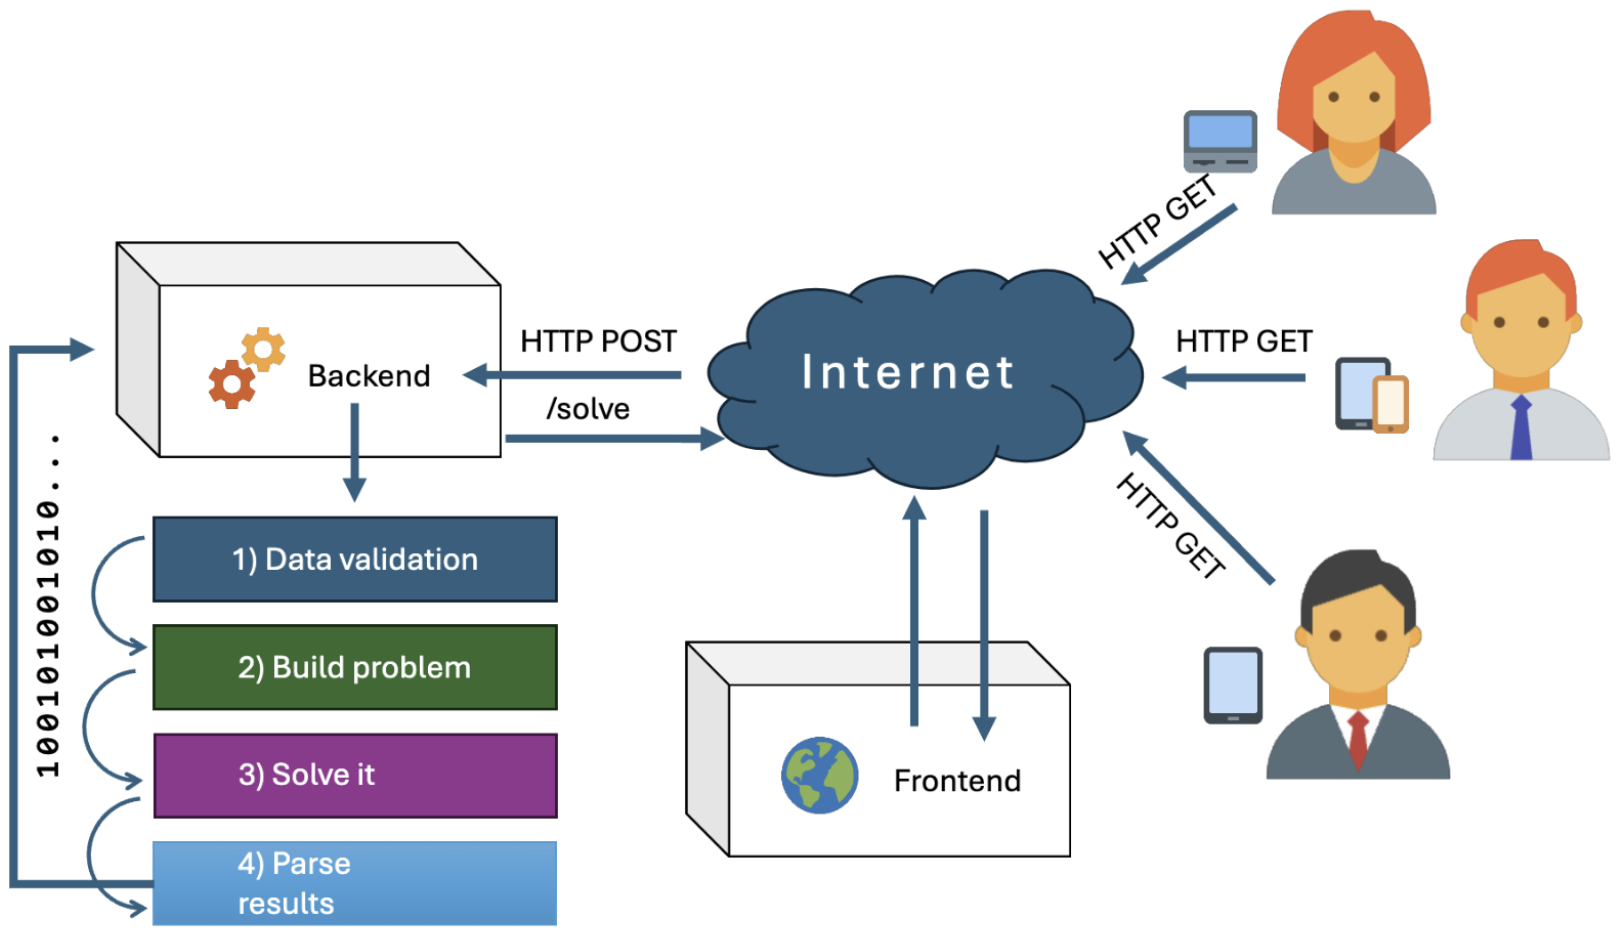
\includegraphics[width=\textwidth]{./images/System_Design.png}
	\caption{System architecture diagram}
	\label{fig:ui_diagram}
\end{figure}

\subsection{Backend - APIs and Solver}
The backend, as previously mentioned, is responsible for receiving the problem instance from the frontend and solving it using the z3-solver. The backend exposes a single endpoint \texttt{/solve} which receives a JSON object containing the problem instance and returns a JSON object with the solution.

This is the structure of a call to the \texttt{/solve} endpoint on the backend started on the local machine:

\begin{verbatim}
curl -X 'POST' \
	'http://localhost:8000/api/v1/solve?n_movers=3&n_floors=3&max_steps=10' \
	-H 'accept: application/json' \
	-H 'Content-Type: application/json' \
	-d '[
		{
		"name": "Table",
		"floor": 1
		},
		{
		"name": "Wardrobe",
		"floor": 2
		}
	]'
\end{verbatim}

The sequence diagram in Figure~\ref{fig:sequence-diagram} illustrates the interaction between a user, the React-app frontend via Custom API, and the backend solver service in a Movers SAT problem-solving application.

\begin{figure}[H]
	\centering
	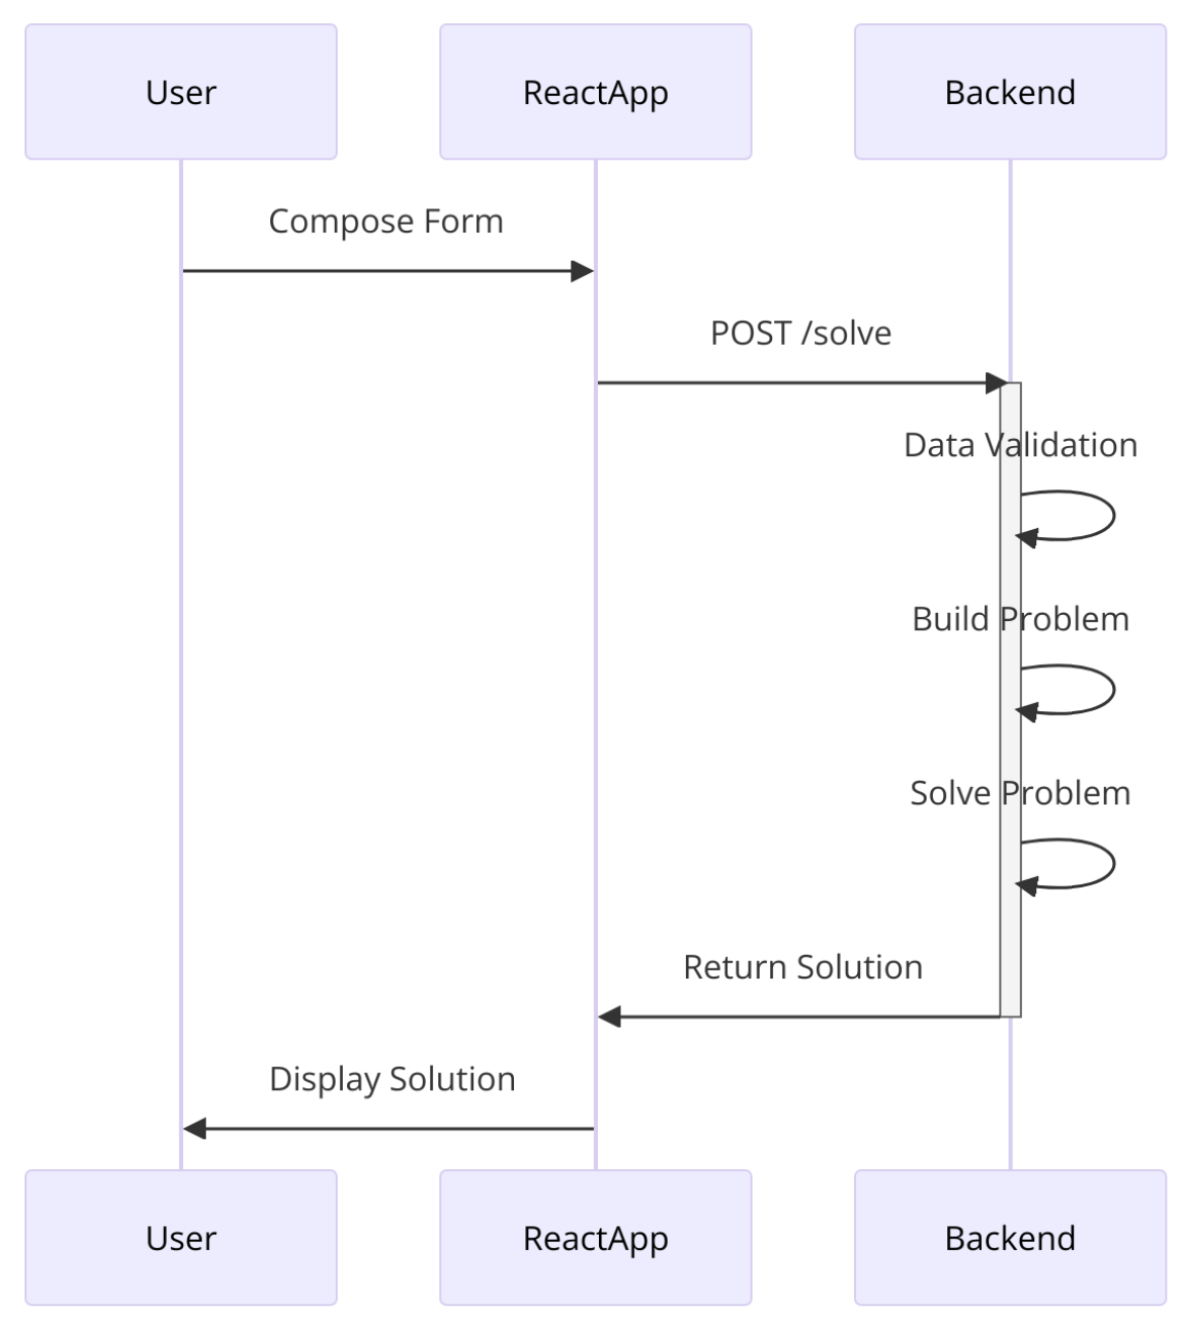
\includegraphics[width=0.5\textwidth]{./images/sequenceDiagram.png}
	\caption{Sequence Diagram}
	\label{fig:sequence-diagram}
\end{figure}

Below is a step-by-step explanation of the process:

\begin{enumerate}

	\item \textbf{Backend Solver Service}:
	      \begin{itemize}
		      \item Upon receiving the request, the backend solver service is activated and begins processing the request.
		      \item \textbf{Data Validation}: The backend performs data validation to ensure that the input parameters (number of movers, floors, maximum steps, and furniture details) are valid and correctly formatted.
		      \item \textbf{Problem Building}: After successful validation, the backend constructs the problem by defining the necessary constraints and setup required to solve the Movers SAT problem.
		      \item \textbf{Problem Solving}: The backend then runs the solver to compute the solution to the problem. This involves calculating the optimal steps and actions needed to move the furniture as specified.
	      \end{itemize}
	\item \textbf{Response to React-app}:
	      \begin{itemize}
		      \item Once the problem is solved, the backend sends the solution back to the React-app. This response includes the computed steps and actions for the movers and furniture.
	      \end{itemize}
	\item \textbf{Display Solution}:
	      \begin{itemize}
		      \item The React-app receives the solution and displays it to the user. The user can now see the detailed steps and actions taken to solve the Movers SAT problem.
	      \end{itemize}
\end{enumerate}

This diagram captures the entire workflow from user input to solution display, highlighting the key interactions and processes involved in solving the Movers SAT problem using the React-app and backend solver service.
\pagebreak

\section{How to Get Started}
This guide will help you to install the tool and run your first network.

\subsection{Requirements}

\begin{itemize}
	\item Python 3.6 or higher
	\item \texttt{pip} (Python package manager) or \texttt{conda} (Anaconda package manager)
\end{itemize}

\subsection{Step 1: Clone the repository}

You can clone the repository using \texttt{git}:

\begin{lstlisting}[language=bash]
# With SSH
git clone git@github.com:lucadibello/movers-sat-problem.git && cd movers-sat-problem
# With HTTPS
git clone https://github.com/lucadibello/movers-sat-problem.git && cd movers-sat-problem
\end{lstlisting}

\subsection{Step 2: Install Python requirements}

To install the required Python packages, you can either use \texttt{pip} (to install the packages globally) or use \texttt{conda} (preferred method) to create a virtual environment and install the packages locally.

\subsubsection*{Option A: Using \texttt{conda}}

\begin{lstlisting}[language=bash]
# Create virtual environment + install packages
conda env create --file=environment.yml
# Activate the virtual environment
conda activate movers
\end{lstlisting}

\subsubsection*{Option B: Using \texttt{pip}}

\begin{lstlisting}[language=bash]
# Install the required packages
pip install -r requirements.txt
\end{lstlisting}

\subsection{Step 3: Run the backend}

\begin{lstlisting}[language=bash]
# Start the backend in production mode
cd ./src/backend && make start
\end{lstlisting}

or, if you want to start the backend in development mode (with \textit{fast refresh}):

\begin{lstlisting}[language=bash]
# Start the backend in development mode
cd ./src/backend && make dev
\end{lstlisting}

\pagebreak

\section{Evaluation}

First of all, we needed to thoroughly understand the problem at hand. To achieve this, we organized a comprehensive discussion involving all team members. This discussion aimed to elucidate the various aspects of the problem, ensuring that everyone had a clear and vivid understanding of the issue. We explored different perspectives, asked clarifying questions, and shared relevant insights, all of which contributed to a more profound and collective grasp of the problem's intricacies. Then we divided into smaller groups so that we could work on frontend and backend at the same time.

\vspace{1em}

\textbf{General Problems:}

\begin{enumerate}
	\item As none of us had prior experience with the z3-solver, we had to spend a considerable amount of time learning how to use it effectively.
	\item We encountered some difficulty in identifying all the edge cases of the problem due to the lack of clarity in certain descriptions.
\end{enumerate}

\textbf{Frontend Problems:}

\begin{enumerate}
	\item Due to our initial unfamiliarity with the React library, we required a considerable amount of time to learn how to utilize it effectively to achieve the desired results.
	\item Offering a user-friendly interface that is both intuitive and easy to use was a significant challenge. We had to ensure that the interface was easy to navigate and that users could input the necessary data without any confusion.
\end{enumerate}

\textbf{Backend Problems:}

\begin{enumerate}
	\item We initially thought that certain constraints were not necessary, but after further analysis, we realized that they were crucial for the problem's correct solution.
	\item The backend API was challenging to implement as it required additional features such as data validation, error handling, and response formatting, features that we initially overlooked.
\end{enumerate}

\end{document}
